% Layout: (_2,_3):(_1,_2)
\documentclass[convert]{standalone}
\usepackage{tikz}

\begin{document}
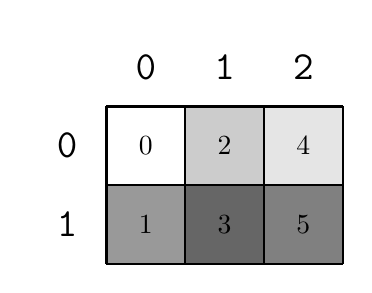
\begin{tikzpicture}[x={(0cm,-1cm)},y={(1cm,0cm)},every node/.style={minimum size=1cm, outer sep=0pt}]

\node[fill=black!00] at (0,0) {0};
\node[fill=black!20] at (0,1) {2};
\node[fill=black!10] at (0,2) {4};
\node[fill=black!40] at (1,0) {1};
\node[fill=black!60] at (1,1) {3};
\node[fill=black!50] at (1,2) {5};
\draw[color=black,thick,shift={(-0.5,-0.5)}] (0,0) grid (2,3);

\node at (0,-1) {\Large{\texttt{0}}};
\node at (1,-1) {\Large{\texttt{1}}};
\node at (-1,0) {\Large{\texttt{0}}};
\node at (-1,1) {\Large{\texttt{1}}};
\node at (-1,2) {\Large{\texttt{2}}};
\end{tikzpicture}
\end{document}
